\chapter{Convolutional Neural Networks}
Convolutional Neural Network is a class of deep, feed-forward neural network, that can be successfully applied to systems with high dimensional input such as images.

It is a pattern recognition mechanisms that is inspired by the way in which mammals visually perceive the world around them using a layered architecture of neurons in the brain. 

Convolutional Neural Networks leverage three ideas:
\begin{enumerate}
\itemsep0em 
\item local connectivity
\item parameter sharing
\item pooling hidden units
\end{enumerate}

CNNs exploit spatially-local correlation by enforcing a local connectivity pattern between neurons of adjacent layers. In other words, each unit in the convolutional hidden layer is not connected with all units in a previous layer, instead it is connected to a subset of units from a previous layer. This approach helps to solve the problem of unmanageable number of parameters. 


The primary purpose of convolution in case of a CNNs is to extract features from the input image. In convolutional layer, the set of filters (typically square matrices with random values) is generated. 

Each filter is replicated across the entire visual field. These replicated units share the same parameterization (weight vector and bias) and form a feature (activation) map. Activation maps indicate ‘activated’ regions, i.e. regions where features specific to the filter have been detected in the input. 

Computation of those feature maps corresponds to computation of discrete convolution of a $i_{th}$ channel of input and filter matrix $W \in \Re^{2h_{1}+1 \times 2h_{2}+1}$. 

The convolution operation is given by
\begin{equation}
(X \ast W)_{r,s} = \sum_{u=-h_{1}}^{h_{1}}\sum_{v=-h_{2}}^{h_{2}} W_{u,v}X_{r+u,s+v}
\end{equation}

\begin{equation}
W =
\left[
\begin{matrix}
w_{-h_{1},-h_{2}} & \cdots & w_{-h_{1},h_{2}}  \\
\vdots & w_{0,0}& \vdots\\
w_{h_{1},-h_{2}} & \cdots & w_{h_{1},h_{2}} 
\end{matrix}
\right]
\end{equation}

The behaviour of this operation towards the borders of the image is handle by 0-padding if needed. 

The $i_th$ feature map in layer $l$ is computer as  

\begin{equation}
z_{i}^{(l)} = \sum_{j=1}^{m} K_{i,j}^{(l)} \ast Y_{j}^{l-1}
\end{equation}
where $m$ is the size of the $l$ layer input.

The output of the layer l, denoted $Y_{i}^{(l)}$ is given by

\begin{equation}
Y_{i}^{(l)} = f\Big(z_{i}^{(l)}\Big)
\end{equation}
where $f$ is an activation function.

The values of the filter matrix change with each learning iteration over the training set, indicating that the network is learning to identify which regions are of significance for extracting features from the data. 

Another important concept of CNNs is max-pooling, which is a form of non-linear down-sampling. Max-pooling partitions the input image into a set of non- overlapping rectangles and, for each such subregion, outputs the maximum value.
Max-pooling is useful in vision for two reasons: 

\begin{itemize}
\itemsep0em 
\item By eliminating non-maximal values, it reduces computation for upper layers.
\item It provides a form of translation invariance.
\end{itemize}

Since it provides additional robustness to position, max-pooling is a “smart” way of reducing the dimensionality.
\\\\\\\\
After a sequence of those operation the output is flattened and applied to the fully connected layer.
At the very end of the network the output is squashed with the softmax layer, so that each element in the output vector corresponds to the probability value for each class.

\begin{equation}
\sigma(o_{j}) = \frac{e^{o_{j}}}{\sum_{k=1}^{K} e^{o_{k}}}
\end{equation}

where $K$ is the number of classes and $o_{j}$ is the $j_{th}$ value of the output vector.

The whole process is presented in the figure (??) 

\begin{figure}[H]
\centering
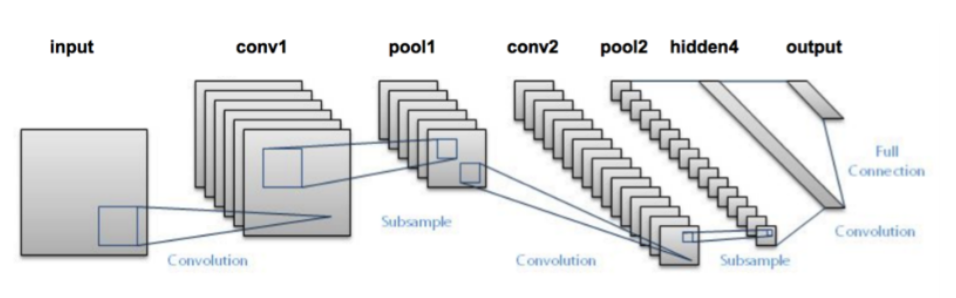
\includegraphics[scale=0.7]{img/proces.png}
\caption{A typical convolutional neural network for face recognition}
\end{figure}

The algorithm is trained with backpropagation. 
The backpropagation algoritihm for convolutional neural networks is slightly more complicated than the one for Multilayered Perception. The general idea is exactly the same, but in CNN we have to face with backpropagation through flatenning, maxpooling and convolution, which requires more effort in practice. 

The first step, as in MLP, is to calculate the error between predicted and expected class probabilities. To do that we calculate the cross entropy error.
Cross entropy measure is widely used when the network output represents the class probabilities. Thus it is used as a loss function in neural networks which have softmax activations in the output layer.


The softmax activation of the ith output unit is: 

\begin{equation}
o_{i} = \frac{e^{s_{i}}}{\sum_{k=1}^{K} e^{s_{k}}}
\end{equation}

where $K$ is the number of classes and $s_{i}$ is the $i_{th}$ value of the last dense layer output vector.

The cross entropy function for multi-class output is given by:

\begin{equation}
E(o, o') = -\sum_{i=1}^K o'_{i} \ln(o_{i})\end{equation} 

\begin{equation}
E = -\sum_{i=1}^K o'_{i} \ln(o_{i})
\end{equation} 

Computing the gradient yields
\begin{equation}
\frac{\partial E}{\partial o_{i}} = -\frac{o'_{i}}{o_{i}}
\end{equation}

\begin{equation}
\begin{split}
\frac{\partial o_i}{\partial s_k}  & = \left\{ \begin{array}{ll}
\frac{e^{s_{i}}}{\sum_{j=1}^{K} e^{s_{j}}} - \Big(\frac{e^{s_{i}}}{\sum_{j=1}^{K} e^{s_{j}}}\Big)^2 & \textrm{$i\neq k$}\\
-\frac{e^{s_{i}} e^{s_{k}}}{(\sum_{j=1}^{K}e^{s_{j}})^2} & \textrm{$i=k$}
\end{array} \right. \\
& = \left\{ \begin{array}{ll}
o_i (1-o_i)& \textrm{$i\neq k$}\\
-o_i o_k & \textrm{$i=k$}
\end{array} \right.
\end{split}
\end{equation}

\begin{equation} 
\begin{split}
\frac{\partial E}{\partial s_i} & = \sum_k^{K} \frac{\partial E}{\partial o_{k}} \frac{\partial o_{k}}{\partial s_{i}} \\
 & = \frac{\partial E}{\partial o_{i}} \frac{\partial o_{i}}{\partial s_{i}} - \sum_{k \neq i} \frac{\partial E}{\partial o_{k}}\frac{\partial o_{k}}{\partial s_{i}}\\
& = o'_{i} (1- o_{i}) + \sum_{k \neq i} o'_{k}o_{i}\\
& = o't_{i} + o_{i} \sum_{k} o'_{k} \\
& = o_{i} - o'_{i}
\end{split}
\end{equation}

The gradient for weight in the last dense layer can be computed as follows:

\begin{equation}
\begin{split}
\frac{\partial E}{\partial w_{ji}} & = \sum_{i}\frac{\partial E}{\partial s_{i}} \frac{\partial s_{i}}{\partial w_{ji}}\\
& = (o_{i} - o'_{i})h_{j}
\end{split}
\end{equation}

where $h_{j}$ is the output of the first dense layer in the network and $w_{ij}$ is the weight connecting the units from second dense layer to the output layer.

The error is backpropagated further as described in chapter 4.3 (??).

The next step is to perform the reversed flatten layer, so that the error can be backpropagated further to maxpooling layer. Backpropagating through maxpooling layer implements the idea that the gradient from the flatten layer is passed back to only that neurons which achieved the maximum value in forward pass during maxpooling computation. All other neurons get zero gradient.

The gradient prepared in such a way is ready to be backpropagated through convolutional layers.
The backpropagation for convolutional layer can be applied as described in chapter 4, however equation 4.12 changes to:

\begin{equation}
\Delta w_{ij} = \lambda z_{j}^{(l-1)} \sum_{k=1}^{m^{(l)}}\delta_k^{(l)}
\end{equation}

As in every other Artificial Neural Network training process can be decomposed in the following steps:

\begin{enumerate}
\itemsep0em 
\item Feed-forward pass
\item Backpropagation of each layer
\item Weight updates
\end{enumerate}

The algorithm is stopped when the value of the error function is sufficiently small.

DeepFace [Taigman et al., 2014] and FaceNet [Schroff, Kalenichenko, and Philbin, 2015] are two of the most successful applications of CNNs in the Face Recognition  problem. These two have provided state-of-art results in recent years, with the best results being obtained by the second one.

\section{Implementation and test results}

The Convolutional Neural Network may differ in number of layers and their connections. The one that was implemented has the following architecture:

\begin{python}
    def forward_pass(self, X):
        h = self.relu(self.cnn_layer(X, layer_i=0, border_mode="full"))
        h = self.relu(self.cnn_layer(h, layer_i=1, border_mode="valid"))
        h = self.maxpooling_layer(h)
        h = self.relu(self.cnn_layer(h, layer_i=3, border_mode="valid"))
        h = self.maxpooling_layer(h)
        h = self.flatten_layer(h)
        h = self.relu(self.dense_layer(h, layer_i=6))
        h = self.dense_layer(h, layer_i=7)
        h = self.softmax_layer2D(h)
        max_i = self.classify(h)
      	return max_i[0]
\end{python}

The first two and the 4th layer in the network performs the convolutional operation followed by activation function RELU.

The input to the network is an image, that can be treated as matrix with three dimensions, each corresponding to every color channel (RGB). In this case every image has the same width and height $k$ equal to 76 pixels. 

\begin{equation}
R =
\left[
\begin{matrix}
r_{11} & r_{21} & \cdots & \cdots & r_{k1}\\
r_{12} & r_{22} & \cdots & \cdots & r_{k2}\\
r_{13} & r_{23} & \cdots & \cdots & r_{k3}\\
r_{14} & r_{24} & \cdots & \cdots & r_{k4}\\
\cdots & \cdots & \cdots & \cdots & \cdots\\
\cdots & \cdots & \cdots & \cdots & \cdots\\
r_{1k} & r_{2k} & \cdots & \cdots & r_{kk}
\end{matrix}
\right]
G =
\left[
\begin{matrix}
g_{11} & g_{21} & \cdots & \cdots & g_{k1}\\
g_{12} & g_{22} & \cdots & \cdots & g_{k2}\\
g_{13} & g_{23} & \cdots & \cdots & g_{k3}\\
g_{14} & g_{24} & \cdots & \cdots & g_{k4}\\
\cdots & \cdots & \cdots & \cdots & \cdots\\
\cdots & \cdots & \cdots & \cdots & \cdots\\
g_{1k} & g_{2k} & \cdots & \cdots & g_{kk}
\end{matrix}
\right]
B =
\left[
\begin{matrix}
b_{11} & b_{21} & \cdots & \cdots & b_{k1}\\
b_{12} & b_{22} & \cdots & \cdots & b_{k2}\\
b_{13} & b_{23} & \cdots & \cdots & b_{k3}\\
b_{14} & b_{24} & \cdots & \cdots & b_{k4}\\
\cdots & \cdots & \cdots & \cdots & \cdots\\
\cdots & \cdots & \cdots & \cdots & \cdots\\
b_{1k} & b_{2k} & \cdots & \cdots & b_{kk}
\end{matrix}
\right]
\end{equation}

In convolutional layer each of those matrices were convolved with each of 32 randomly chosen filters. The convolutional layer has an additional parameter \textit{border mode}, which can be set to either \textit{full} or \textit{valid}, which defines if the convolution operation involves padding around the input (valid border mode sets padding to $0$).
The convolution across each channel is summed up. As a result first two layers we obtain a matrix with dimensions = $(1, 32, 76, 76)$.


The 3rd and the 5th layer are maxpooling layers, which purpose is to reduce the dimensionality of the data. No activation function is applied. The 3rd and 5th output matrix dimensions are accordingly: $(1, 32, 38, 38)$ and $(1, 32, 18, 18)$.

One of the last stages of a convolutional neural network (CNN) is a dense layer. It's just a simple MLP layer, as described in chapter(??). It requires the one-dimensional input - the output of convolutional layers has to be converted into a 1D feature vector. This operation is called flattening and is performed with the flatten layer. 
After flattening the data we obtain a vector with $10368 (18*18*32)$ elements. The MLP layer used in this example has one hidden layer with $6000$ units. The output layer consist of number of units equals to the number of classes (amount of people in the database) - in our case $20$. 

The last part of the network is a softmax layer, which allows us to calculate the probability value for each class.

The above construction allows to classify an image only if the filter parameters and dense layer parameters are set correctly. The choice of those coefficients is made randomly and they are trained with backpropagation algorithm. 

During the algorithm implementation it turned out that training the entire network on a reasonably sized dataset would be unfeasible on a personal laptop. Even though the dimensionality reduction (maxpooling)is applied, the total number of parameters that need to be trained is equal to ~ $1,25*10^9$. 

According to the convolutional networks theory we know that the goal of the lower layers is to identify lower-level features such as colors, shapes or textures, and only the top layers distinguish the specific, higher-level features of each class. Based on this idea, instead of training the whole convolutional network, we can take an existing convolutional network model and train the last layer of the network so that it can recognize the given data. 

The first experiment was performed with Google Inception-v3 model. The Inception v3 model has nearly 25 million parameters and uses 5 billion multiply-add operations for classifying a single image.

\begin{figure}[H]
\centering
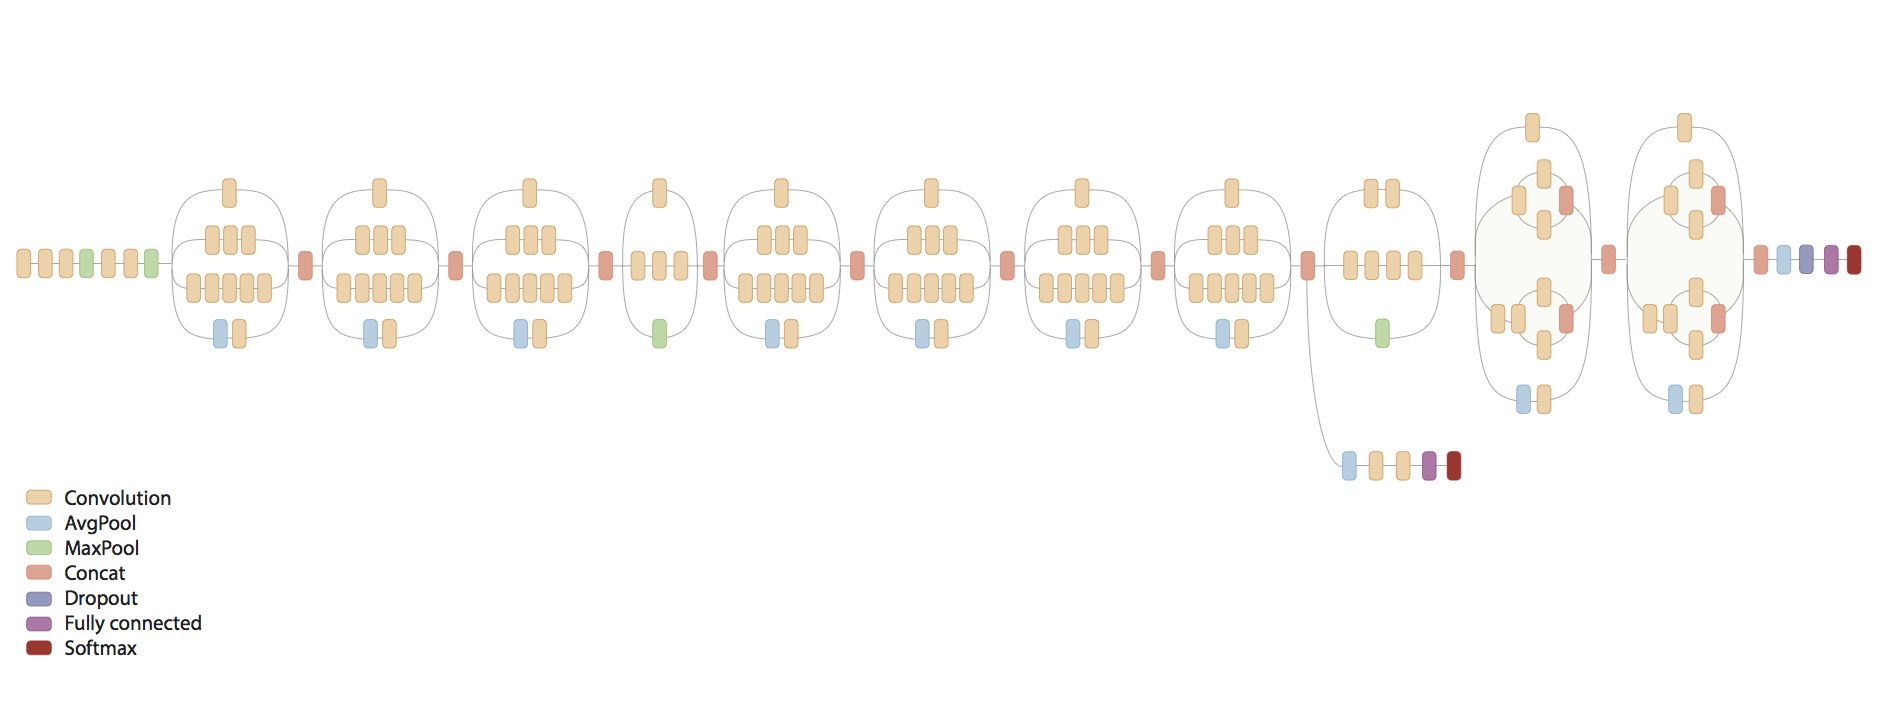
\includegraphics[scale=0.5]{img/inception_v3_architecture.png}
\caption{Google Inception v3 model architecture}
\end{figure}

This model structure is much more complicated than the general convolutional network architecture. Instead of applying all convolutional, maxpooling and dense layers one by one, some of the layers consist of the composition of those operation. The model was trained on ImageNet database with 1000 image categories and turns out to outperform the human recognition abilities. The goal of this experiment is to find out how good this model can be adjusted to recognize human faces, taking into account that there was no facial images in its training data set. 

The tensofflow library provides the function that returns  the outputs from a different layers. We take the last layer with 2048 neurons and connect it to the fully connected layer, creating a new output with amount of neurons corresponding to the amount of individuals in the dataset. To train only a single layer, we specify the list of trainable variables in the training operation. The network will train only the parameters that connects the 2048 inception neurons with 10 output neurons of our network. At the end the softmax activation function is applied in order to calculate probabilities for each class.


\section{Test results}

Algorithm was implemented in Python 3.4 with usage of numpy and tensorflow libraries. 

The test was performed on 10 individuals with the biggest amount of images from Labeled Faces in Wild database. 

\begin{table}[H]
	\centering
	\caption{List of individuals taken for testing the algorithm}
    \begin{tabular}{ | l | l |}
    \hline
    \rowcolor{lightgray}
    Name &  Number of pictures \\ \hline
	George W. Bush & $100$\\  \hline  
	Colin Powell & $100$ \\ \hline    
	Tony Blair & $100$\\\hline
    Donald Rumsfeld  & $100$ \\ \hline
    Gerhard Schroeder  & $100$\\ \hline
    Ariel Sharon &  $77$  \\ \hline
	Hugo Chavez & $71$\\\hline
    Junichiro Koizumi  & $60$\\\hline    
    Jean Chretien  & $55$\\\hline
    John Ashcroft  & $53$\\
    \hline
    \end{tabular}
\end{table}

Data was randomly separated into three sets:
\begin{itemize}
\itemsep0em 
\item 75\% training set
\item 5\% validation set
\item 20\% testing set
\end{itemize}

The algorithm implements early stopping approach. It requires periodically testing the network on a validation set to obtain the score on the cost function (average cross entropy). If the loss does not decrease for a specified number of iterations, training is interrupted. It prevents the network from overfitting. 

The test results visualization were generated by tensorboard module (from tensorflow library).

\begin{figure}[H]
\centering
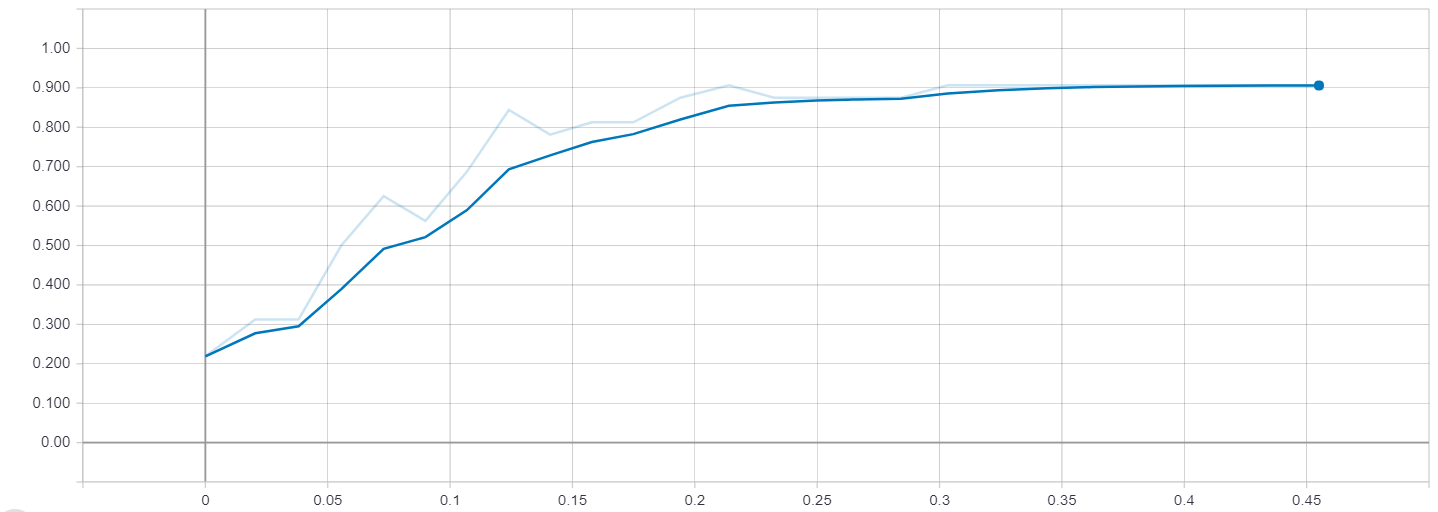
\includegraphics[scale=0.5]{img/train_acc.png}
\caption{Training accuracy}
\end{figure}

\begin{figure}[H]
\centering
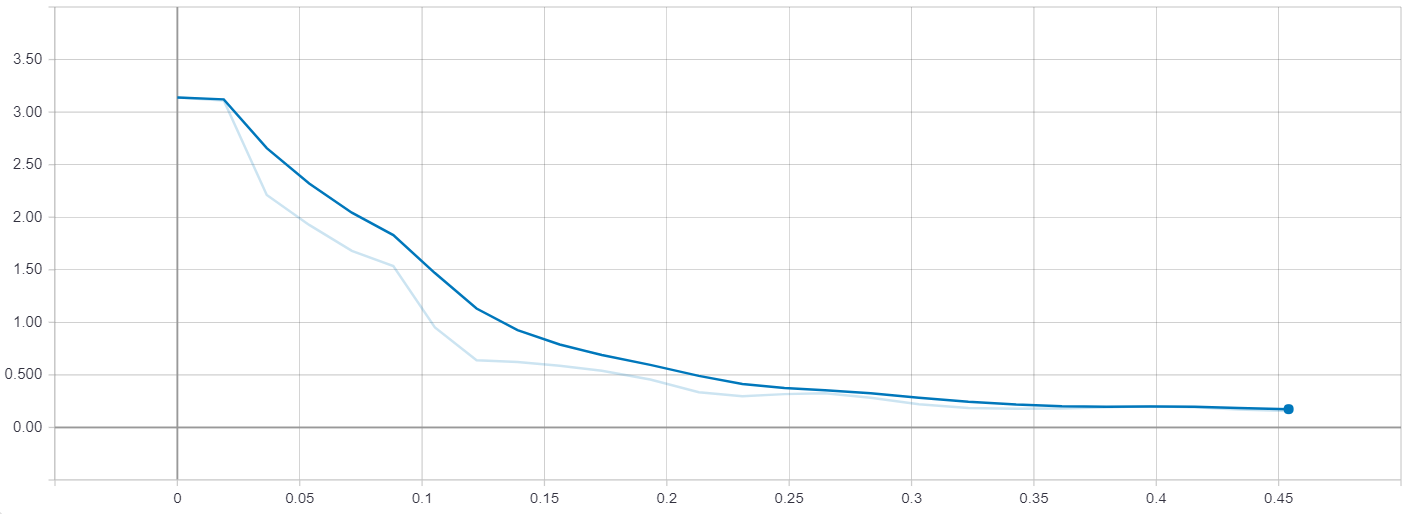
\includegraphics[scale=0.5]{img/valid_loss.png}
\caption{Validation loss}
\end{figure}

Taking into account that these results were obtained via training only last layer of the network, we can consider them better than expected. The training accuracy reached ~80\%.

The recognition rate obtained from testing data set was 83,8\%.

The Chicago Face Database was not tested due to not enough training data that is required for this algorithm. 
